\section{Desenvolvimento}

Este capítulo detalha os processos que ocoreram no desenvolvimento da pesquisa, mostrando os passos seguidos para alcançar os objetivos propostos. Além disso, são abordadas as dificuldades enfrentadas e as adptações e refinamentos realizados ao longo do percurso.

\subsection{Circuito}

\subsubsection{Emissor}

O circuito que permite ``transformar" os bits em luz é composto por um led de alto brilho, um transistor TIP122, dois resistores e uma bateria.

O transistor é ligado como chave na SBC para permitir acionar cargas elétricas da qual a SBC não seria capaz, pois pode fornecer no máximo 16 mA (miliampere) \citeonline{correnteSbc} e como o led de alto brilho consome uma corrente de 18.8mA, uma ligação direta na GPIO (General Purpose Input/Output) poderia queimar a SBC.

\begin{figure}[!htbp]
  \caption{Esquema do circuito emissor}
  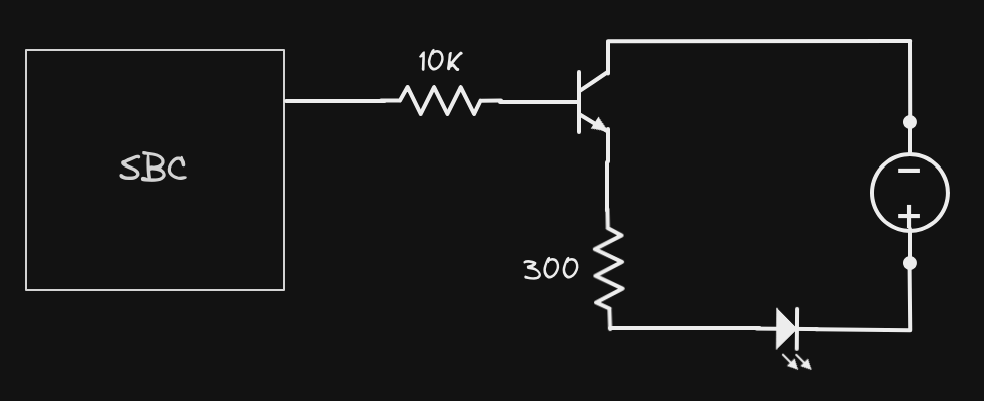
\includegraphics[width=0.5\textwidth]{images/esquema_circuito_emisor.png}
  \legend{Fonte: Autor}
  \label{esquema-circuito-emissor}
\end{figure}

\begin{figure}[!htbp]
  \caption{Esquema do circuito emissor}
  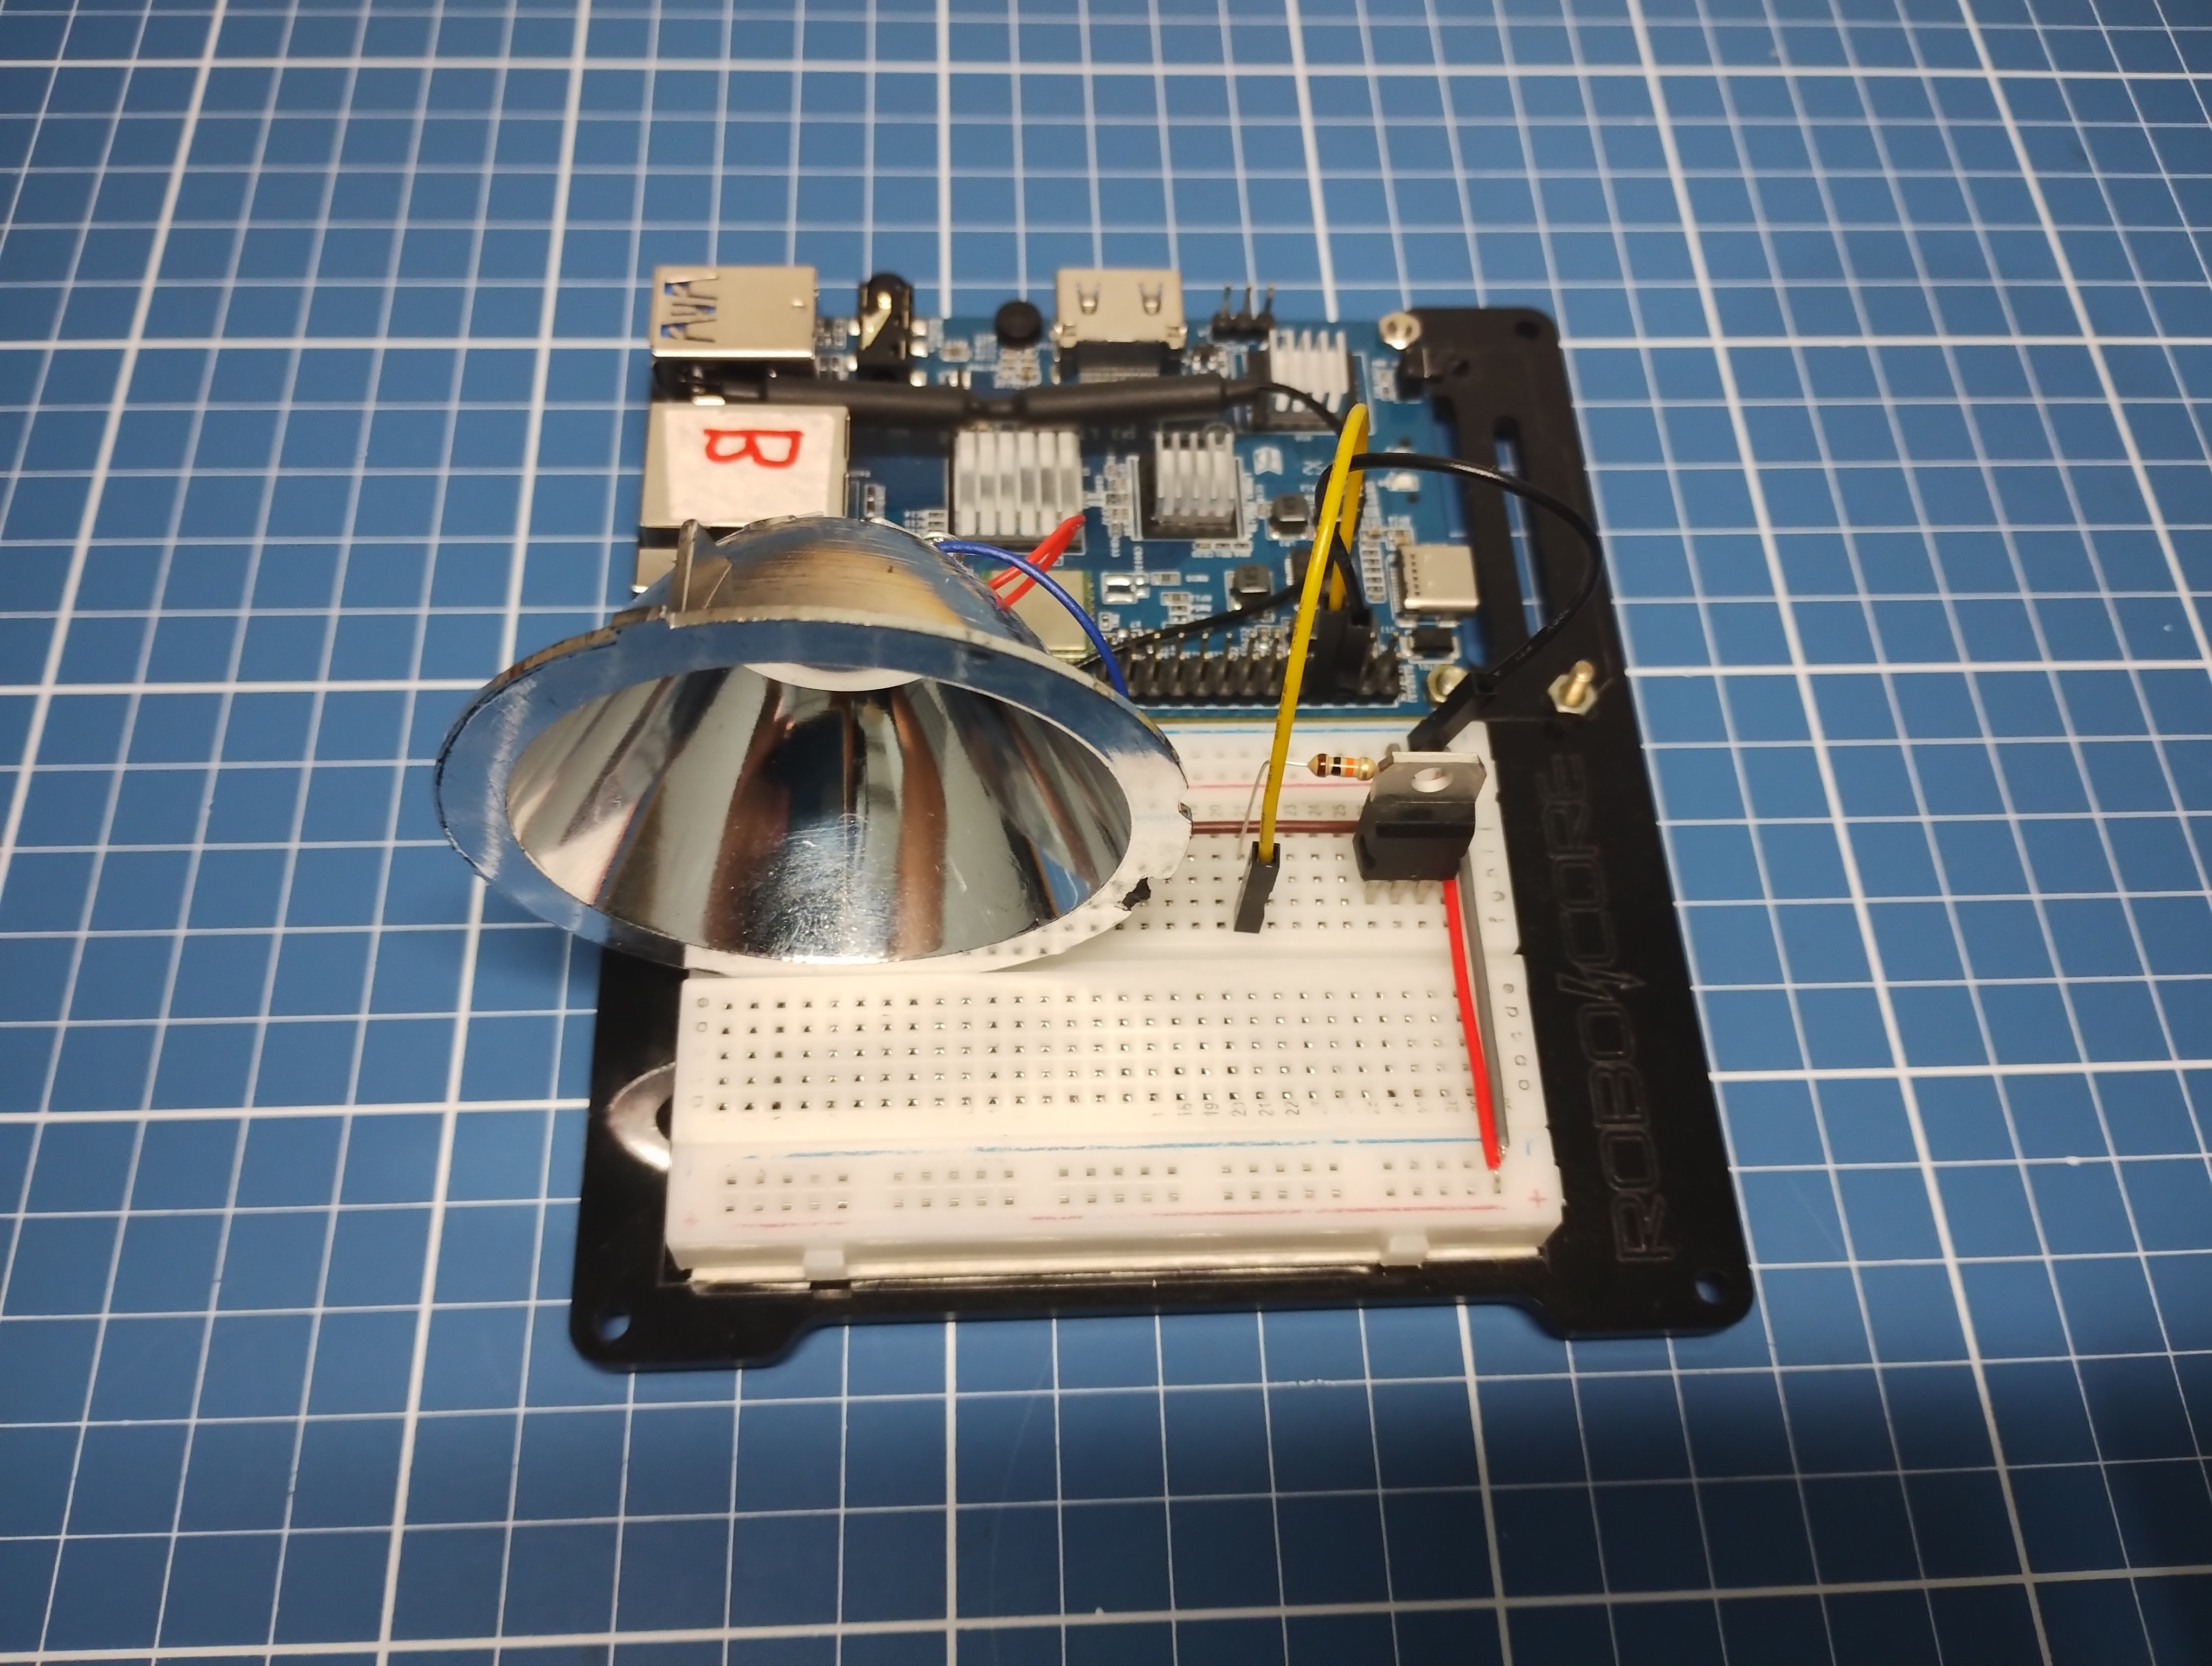
\includegraphics[width=0.4\textwidth]{images/foto_circuito_emisor.jpg}
  \legend{Fonte: Autor}
  \label{foto-circuito-emissor}
\end{figure}

\begin{figure}[!htbp]
  \caption{Consumo do led usado no circuito emissor}
  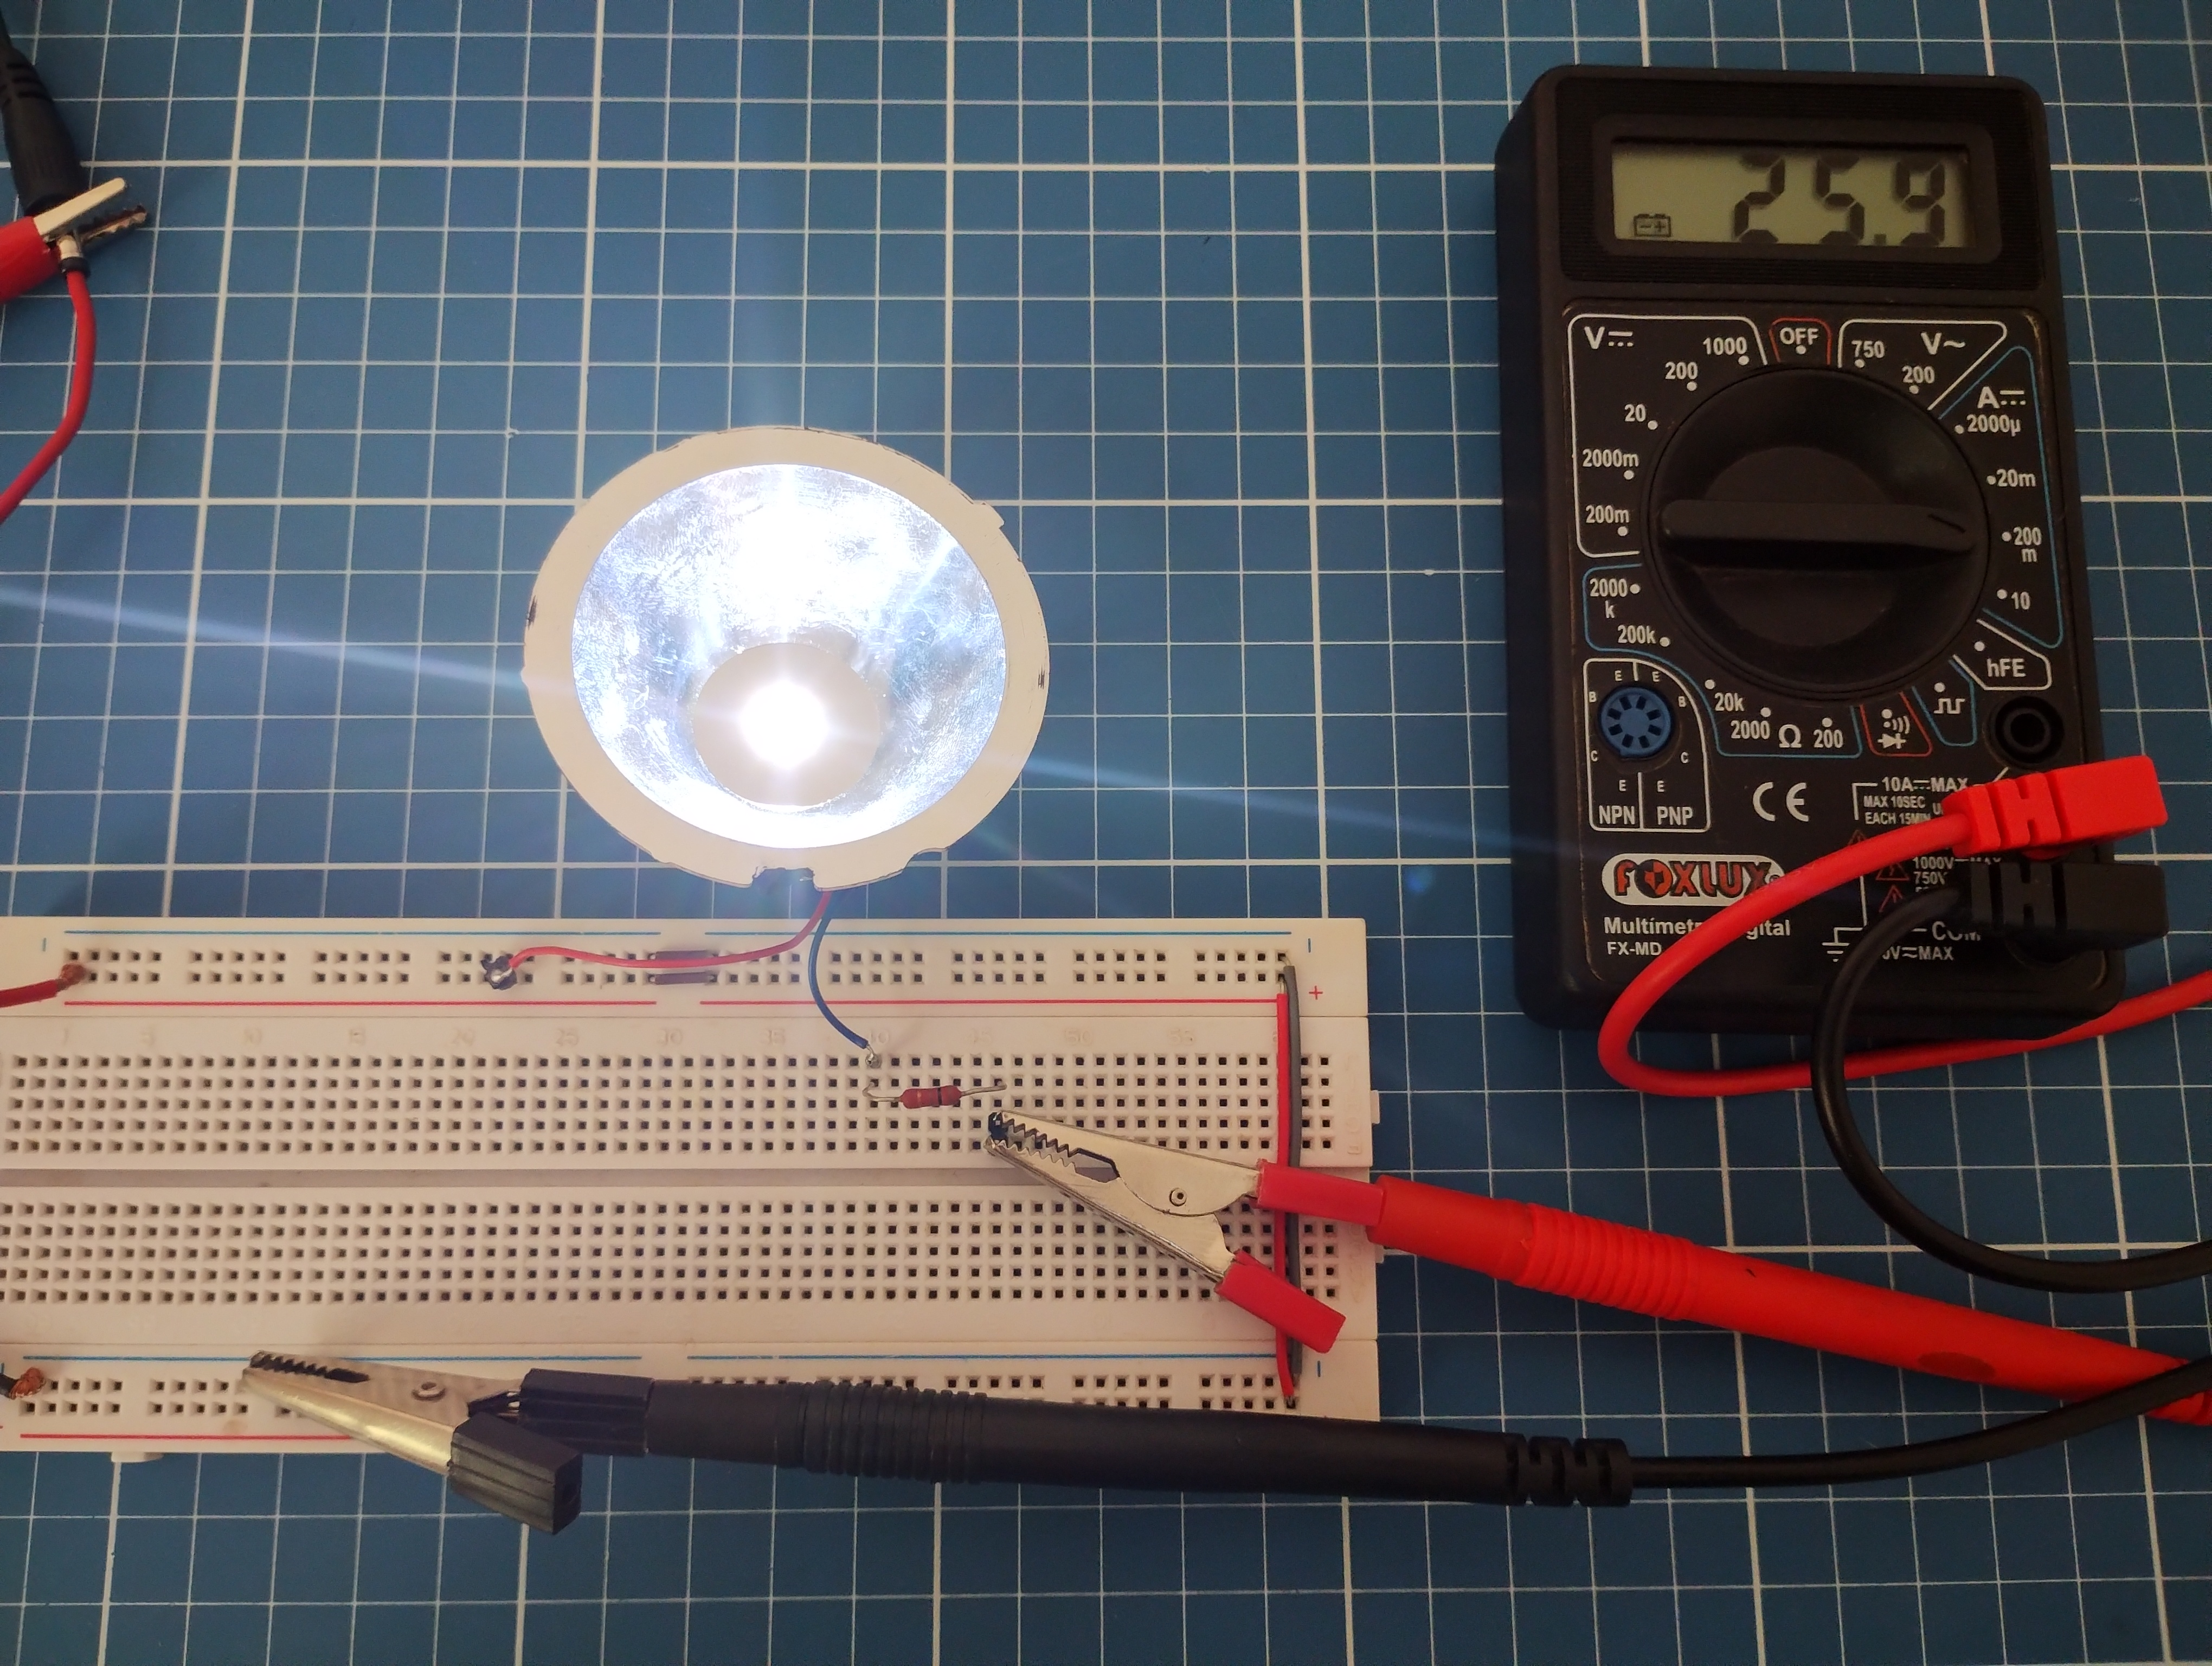
\includegraphics[width=0.4\textwidth]{images/consumo_led.jpg}
  \legend{Fonte: Autor}
  \label{corrente_led}
\end{figure}


\subsubsection{Receptor}

O circuito para receber as informações do emissor é composto por um LDR (Light Dependent Resistor) e um potenciômetro ligado em série. Este circuito permite ler os \emph{bytes} independente da intensidade da iluminação externa, ajustando a posição do potenciômetro.

\begin{figure}[!htbp]
  \caption{Esquema do circuito receptor}
  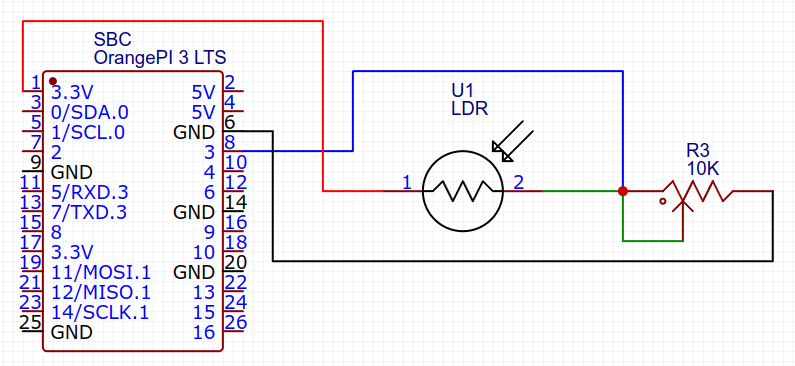
\includegraphics[width=0.5\textwidth]{images/esquema_circuito_receptor.png}
  \legend{Fonte: Autor}
  \label{esquema-circuito-receptor}
\end{figure}


\begin{figure}[!htbp]
  \caption{Esquema do circuito receptor}
  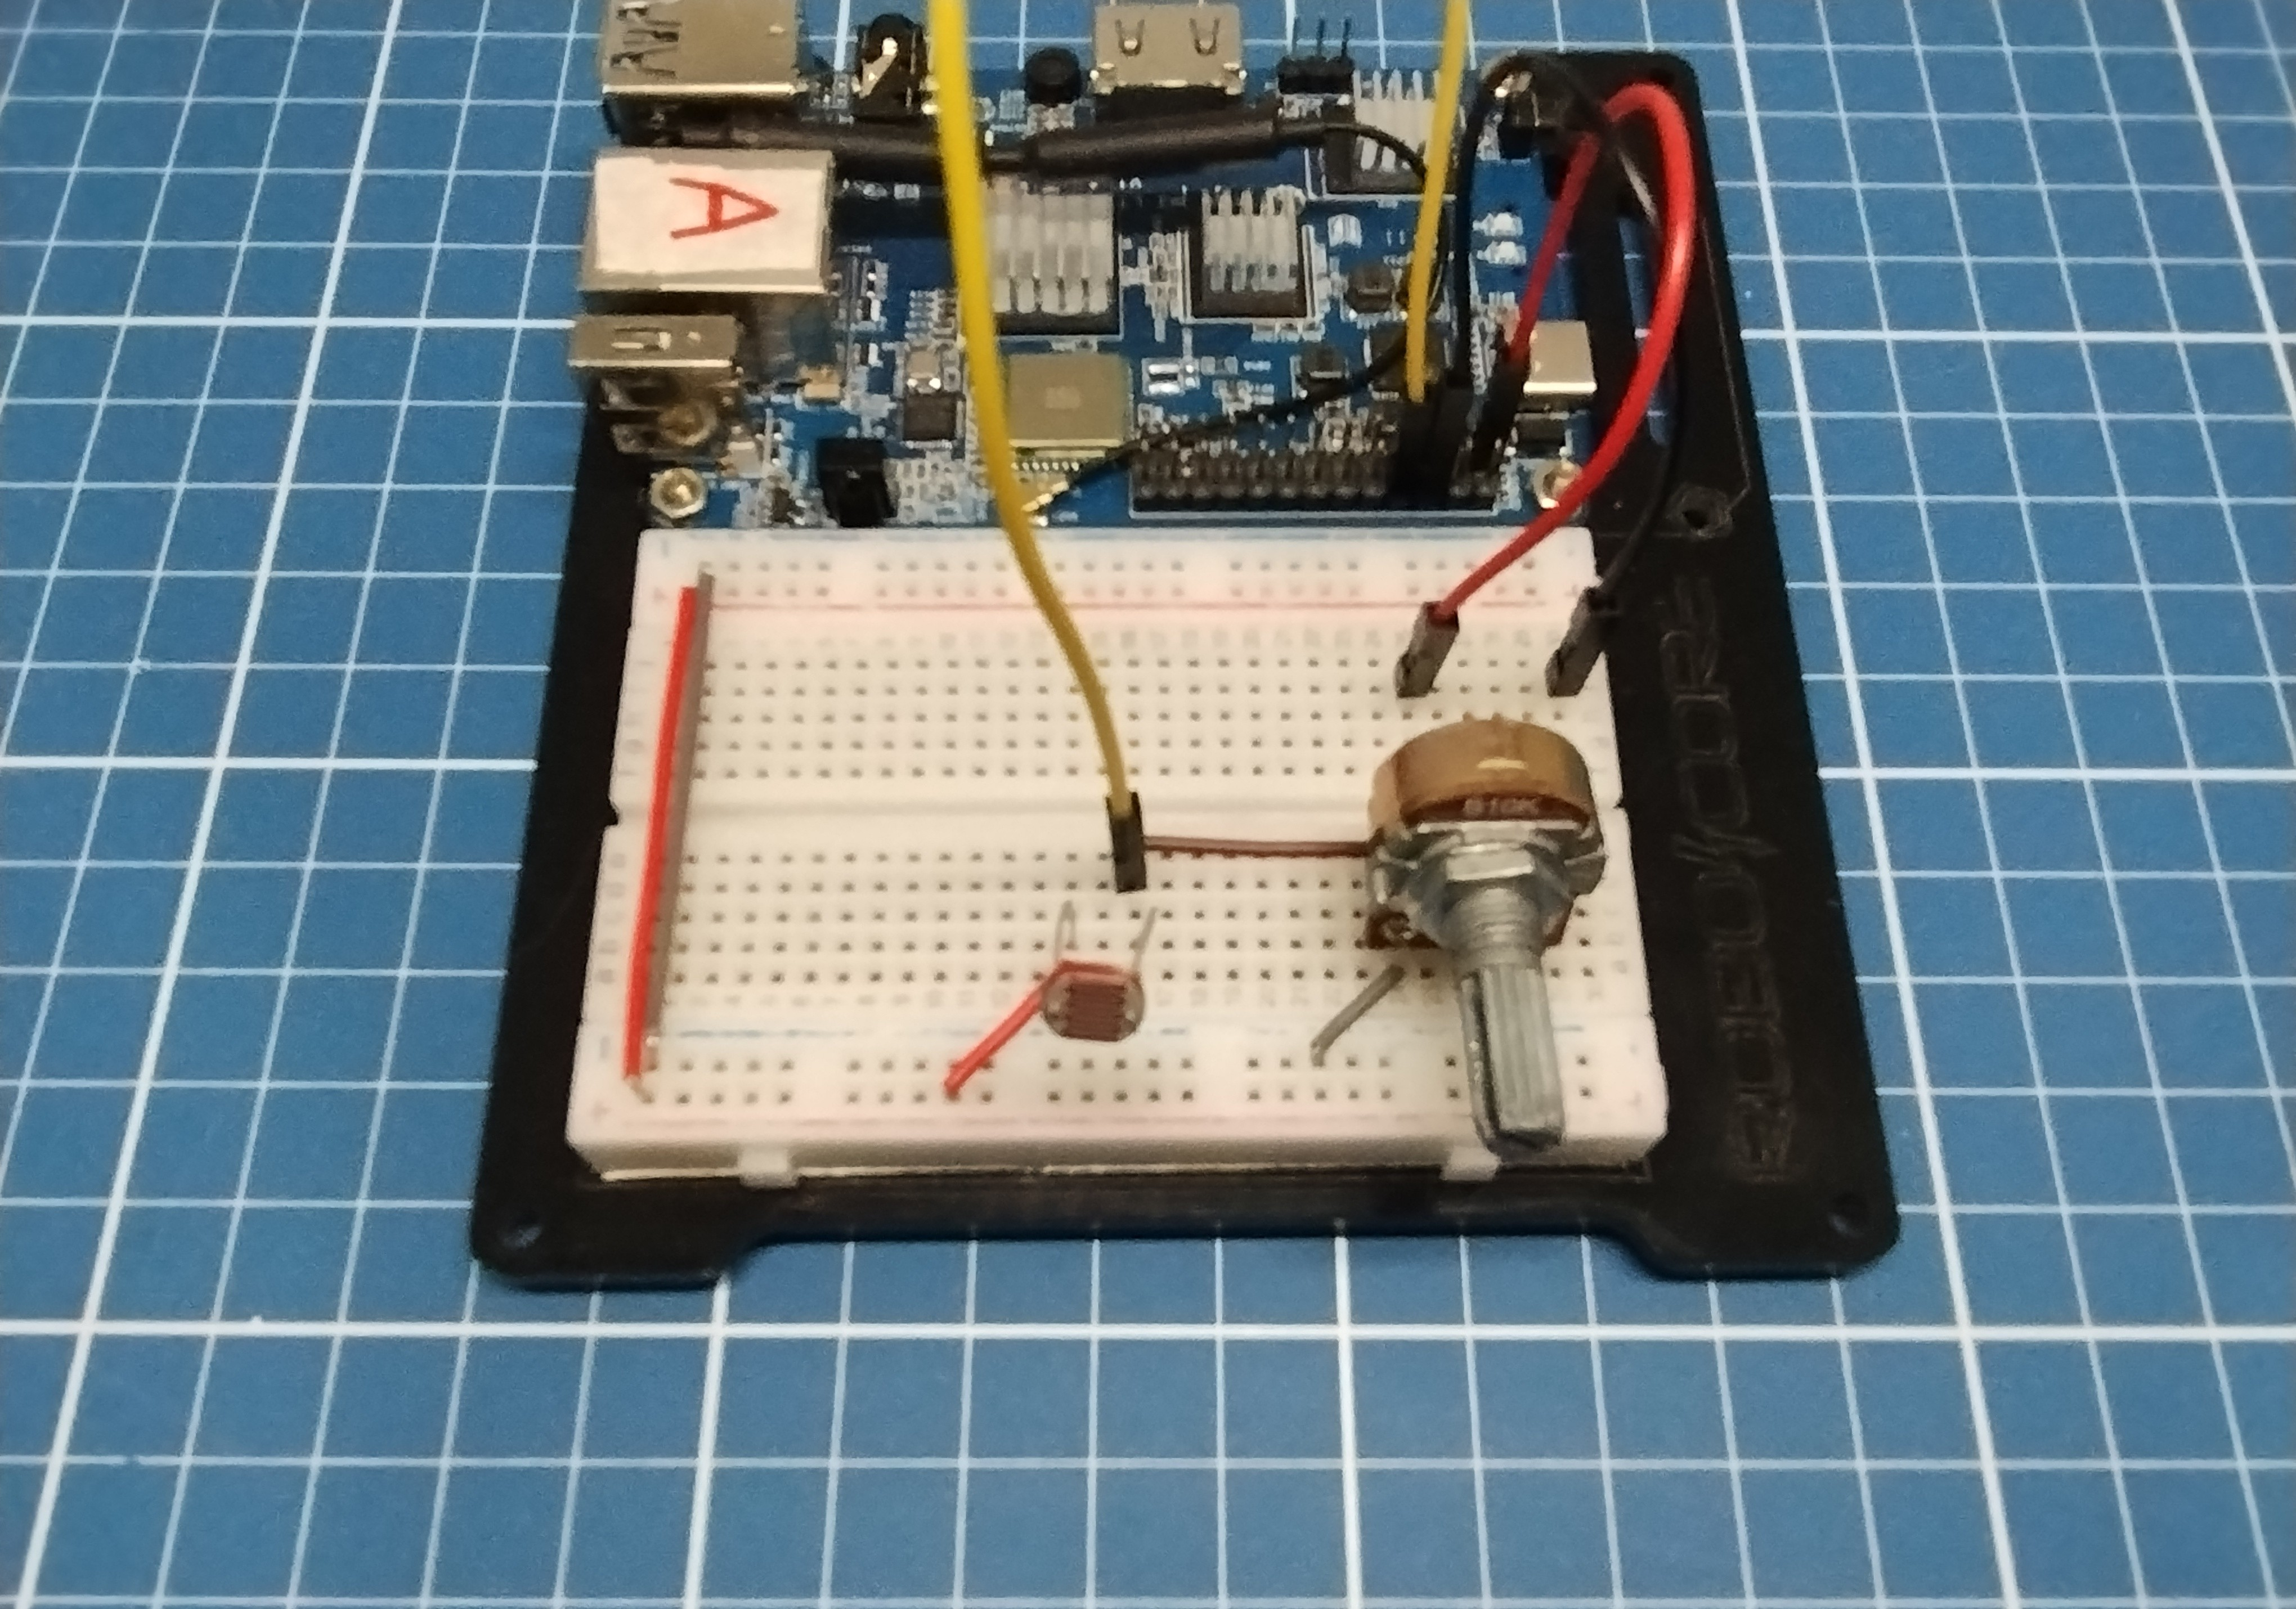
\includegraphics[width=0.4\textwidth]{images/foto_circuito_receptor.jpg}
  \legend{Fonte: Autor}
  \label{foto-circuito-receptor}
\end{figure}

